\documentclass[../main.tex]{subfiles}

\begin{document}

\section*{第1問}

\begin{proof}[解]
$f(x)=1-\cos x-x\sin x=1-C-xS$（$C=\cos x,\ S=\sin x$）とおく。

\textbf{(1)} $f'(x)=S-S-xC=-xC$。$0<x<\dfrac\pi2$で$C>0$より$f'(x)<0$，$x=\dfrac\pi2$で$f'=0$，$\dfrac\pi2<x<\pi$で$C<0$より$f'(x)>0$。よって$f$は$[0,\pi/2]$で減少，$[\pi/2,\pi]$で増加。
\begin{align*}
f(0)=0,\qquad f\Bigl(\frac\pi2\Bigr)=1-\frac\pi2<0,\qquad f(\pi)=1-(-1)-0=2.
\end{align*}
$f(0)=0$かつ$(0,\pi/2)$で$f$は狭義単調減少だから$(0,\pi/2)$に解はなく，$[\pi/2,\pi]$では$f$が$1-\pi/2<0$から$2>0$へ狭義単調増加するので中間値の定理よりただ1つの解$\alpha\in(\pi/2,\pi)$を持つ。よって$0<x<\pi$で$f(x)=0$はただ1つの実解を持つ。

\textbf{(2)} (1)より$0\le x\le\alpha$で$f(x)\le0$，$\alpha\le x\le\pi$で$f(x)\ge0$だから
\begin{align*}
J=-\int_0^\alpha f(x)dx+\int_\alpha^\pi f(x)dx.\tag{①}
\end{align*}
$f$の原始関数の1つを$F(x)$とすると
\begin{align*}
F(x)=\int f(x)dx=x-S-(-xC+S)=x(1+C)-2S
\end{align*}
であり，$F(0)=0$，$F(\pi)=\pi(1+(-1))-0=0$だから
\begin{align*}
J=F(\pi)+F(0)-2F(\alpha)=-2F(\alpha)=-2\alpha(1+\cos\alpha)+4\sin\alpha.
\end{align*}
一方，$f(\alpha)=0$より$\cos\alpha=1-\alpha\sin\alpha$（②）だから，これを代入して
\begin{align*}
J=-2\alpha(2-\alpha\sin\alpha)+4\sin\alpha=2\alpha^2\sin\alpha-4\alpha+4\sin\alpha.
\end{align*}

\textbf{(3)} $K=\dfrac{J-\sqrt2}{\sqrt2}$とおく。(2)の結果より
\begin{align*}
K=\sqrt2\alpha^2\sin\alpha-2\sqrt2\alpha+2\sqrt2\sin\alpha-1.\tag{③}
\end{align*}
②と$\sin^2\alpha+\cos^2\alpha=1$より$\sin^2\alpha+(1-\alpha\sin\alpha)^2=1$，整理して
\begin{align*}
(\alpha^2+1)\sin^2\alpha-2\alpha\sin\alpha=0.
\end{align*}
$0<\alpha<\pi$より$\sin\alpha\neq0$なので，両辺を$\sin\alpha$で割って
\begin{align*}
(\alpha^2+1)\sin\alpha=2\alpha.\tag{④}
\end{align*}
③に④を用いると
\begin{align*}
K=\sqrt2\bigl[(\alpha^2+1)\sin\alpha-2\alpha\bigr]+2\sqrt2\sin\alpha-1-2\sqrt2\sin\alpha+2\sqrt2\sin\alpha
\end{align*}
すなわち，$\sqrt2\alpha^2\sin\alpha-2\sqrt2\alpha=\sqrt2[(\alpha^2+1)\sin\alpha-2\alpha]=\sqrt2\cdot0=0$（④より）だから
\begin{align*}
K=2\sqrt2\sin\alpha-1.
\end{align*}
（③の$\sqrt2\alpha^2\sin\alpha-2\sqrt2\alpha$の部分が④によって消え，$2\sqrt2\sin\alpha-1$のみ残る。）

さて，(1)の増減表と$f\Bigl(\dfrac{3\pi}4\Bigr)=1+\dfrac{\sqrt2}2-\dfrac{3\sqrt2}8\pi>0$（実際$1+\frac{\sqrt2}2\approx1.71$，$\frac{3\sqrt2}8\pi\approx1.67$）から，$f$は$[\pi/2,\pi]$で単調増加で$f(\alpha)=0$，$f(3\pi/4)>0$なので$\alpha<\dfrac{3\pi}4$。よって$\dfrac\pi2<\alpha<\dfrac{3\pi}4$。この範囲で$\sin\alpha$は単調減少だから
\begin{align*}
\sin\alpha>\sin\frac{3\pi}4=\frac{\sqrt2}2.
\end{align*}
したがって
\begin{align*}
K=2\sqrt2\sin\alpha-1>2\sqrt2\cdot\frac{\sqrt2}2-1=2-1=1>0.
\end{align*}
$K=\dfrac{J-\sqrt2}{\sqrt2}>0$より$J>\sqrt2$。
\end{proof}

\newpage

\section*{第2問}

\begin{proof}[解]
方程式
\begin{align*}
x=\Bigl[\frac12\Bigl(x+\frac ax\Bigr)\Bigr]\tag{$\ast$}
\end{align*}
の右辺は整数だから，解$x$は正の整数である。$x=k_a$（$k_a\in\mathbb N$）が解のとき，$k_a\le\dfrac12\Bigl(k_a+\dfrac a{k_a}\Bigr)<k_a+1$，すなわち
\begin{align*}
k_a^2\le a<k_a^2+2k_a.
\end{align*}
これは$a<(k_a+1)^2-1$と同値だから$k_a+1>\sqrt{a+1}$，すなわち$k_a>-1+\sqrt{a+1}$。まとめると
\begin{align*}
-1+\sqrt{a+1}<k_a\le\sqrt a.\tag{$P(a)$}
\end{align*}
したがって，$(\ast)$が解を持つことと，区間$(-1+\sqrt{a+1},\sqrt a\,]$に正の整数が存在することは同値である。

\textbf{(1)} $a=7$：$P(7)$は$-1+2\sqrt2<k_a\le\sqrt7$，すなわち$1.83\cdots<k_a\le2.64\cdots$。$k_a=2$が適し，解は$x=2$。

$a=8$：$P(8)$は$2<k_a\le2\sqrt2=2.82\cdots$。これをみたす整数はない。よって解なし。

$a=9$：$P(9)$は$-1+\sqrt{10}<k_a\le3$，すなわち$2.16\cdots<k_a\le3$。$k_a=3$が適し，解は$x=3$。

\textbf{(2)} $t\in\mathbb N$とする。$t^2\le a<(t+1)^2$のとき$[\sqrt a\,]=t$である。
\begin{itemize}
\item $t^2\le a\le(t+1)^2-2=t^2+2t-1$のとき，$1+a\le(t+1)^2-1<(t+1)^2$より$-1+\sqrt{1+a}<t$（等号は不成立）となり，$t$は$P(a)$をみたす。
\item $a=(t+1)^2-1=t^2+2t$のとき，$-1+\sqrt{1+a}=-1+(t+1)=t$となり，$P(a)$の左側が等号（非成立）になるため，$t$は$P(a)$をみたさない。また$\sqrt a<t+1$より$P(a)$をみたす整数は$t$以外になく，この$a$では$(\ast)$は解を持たない。
\end{itemize}
よって，$(\ast)$が解を持たないのは$a=t^2+2t\ (=(t+1)^2-1)$（$t\in\mathbb N$）と表せるときであり，
\begin{align*}
a_1=1^2+2\cdot1=3,\qquad a_2=2^2+2\cdot2=8.
\end{align*}
（$a=8$が解なしという(1)の結果とも一致する。）一般に$a_n=n^2+2n=n(n+2)$。

\textbf{(3)} $S_n=\displaystyle\sum_{k=1}^n\frac1{a_k}$とおくと，$a_k=k(k+2)$より部分分数分解$\dfrac1{k(k+2)}=\dfrac12\Bigl(\dfrac1k-\dfrac1{k+2}\Bigr)$を用いて
\begin{align*}
S_n=\sum_{k=1}^n\frac1{k(k+2)}=\frac12\sum_{k=1}^n\Bigl(\frac1k-\frac1{k+2}\Bigr)=\frac12\Bigl(1+\frac12-\frac1{n+1}-\frac1{n+2}\Bigr)\xrightarrow[n\to\infty]{}\frac12\Bigl(1+\frac12\Bigr)=\frac34.
\end{align*}
よって$\displaystyle\sum_{n=1}^\infty\frac1{a_n}=\frac34$。
\end{proof}

\newpage

\section*{第3問}

\begin{proof}[解]
$n$枚から2枚を取り出す場合の数は$\binom n2$通りで，これらは同様に確からしい。

$n=3k+2$（$k\in\mathbb N$）のとき，2枚のうち小さい方が$3t$（$t=1,\dots,k$）である場合，大きい方は$3t+1,3t+2,\dots,3k+2$のいずれかだから，その場合の数は
\begin{align*}
P_k(t)=(3k+2)-3t.
\end{align*}
よって，小さい方が3の倍数であるすべての場合の数$N_k$は
\begin{align*}
N_k=\sum_{t=1}^kP_k(t)=k(3k+2)-3\cdot\frac{k(k+1)}2=\frac12k(3k+1)
\end{align*}
となり，もとめる確率は
\begin{align*}
p(3k+2)=\frac{N_k}{\binom{3k+2}2}=\frac{\frac12k(3k+1)}{\frac{(3k+2)(3k+1)}2}=\frac k{3k+2}.
\end{align*}

\textbf{(1)} $n=8=3\cdot2+2$より$k=2$として
\begin{align*}
p(8)=\frac2{3\cdot2+2}=\frac28=\frac14.
\end{align*}

\textbf{(2)} 上で示した通り
\begin{align*}
p(3k+2)=\frac k{3k+2}.
\end{align*}
\end{proof}

\newpage

\section*{第4問}

\begin{proof}[解]
$a>0$とする。$P=(x,y)\neq A$とし，$\overrightarrow{AP}=(x-a,y)$とおく。半直線$AP$上の点$Q$で$\dfrac{AQ}{AP}=t$（$0\le t\le2$）となるものは
\begin{align*}
\overrightarrow{AQ}=t(x-a,y),\qquad Q=(a+t(x-a),\,ty)
\end{align*}
と表せる。条件は，この範囲のすべての$t$に対して
\begin{align*}
\frac{QP}{OQ}\le\frac{AP}{OA}\quad(OQ\neq0)
\end{align*}
が成り立つことである。$QP=|1-t|\cdot AP$，$OA=a$だから，条件は（$AP>0$より）
\begin{align*}
a|1-t|\le OQ=\sqrt{(a+t(x-a))^2+(ty)^2}\qquad(0\le t\le2).
\end{align*}
両辺とも非負なので2乗して整理すると
\begin{align*}
a^2(1-t)^2\le(a+t(x-a))^2+t^2y^2
\end{align*}
\begin{align*}
\Longleftrightarrow\ t\bigl[(x^2-2ax+y^2)t+2ax\bigr]\ge0.\tag{①}
\end{align*}
（展開の詳細：右辺$-$左辺を計算すると$t^2\{(x-a)^2+y^2-a^2\}+t\cdot2ax=t^2(x^2-2ax+y^2)+2axt$となる。）

$t=0$のとき①は自明に成立するから，$t\in(0,2]$で$h(t):=(x^2-2ax+y^2)t+2ax\ge0$が成り立てばよい。$h$は$t$の1次式（線形）だから，区間$[0,2]$上で$h\ge0$となるための必要十分条件は両端点で$h\ge0$となることである（線形関数の値は端点の値の凸結合として得られるため）：
\begin{align*}
h(0)=2ax\ge0,\qquad h(2)=2(x^2-ax+y^2)\ge0.
\end{align*}
$a>0$より$h(0)\ge0\iff x\ge0$。また$h(2)\ge0\iff x^2-ax+y^2\ge0\iff\Bigl(x-\frac a2\Bigr)^2+y^2\ge\Bigl(\frac a2\Bigr)^2$。

以上から，条件をみたす$(x,y)$の範囲は
\begin{align*}
x\ge0\quad\text{かつ}\quad\Bigl(x-\frac a2\Bigr)^2+y^2\ge\Bigl(\frac a2\Bigr)^2,
\end{align*}
すなわち，線分$OA$を直径とする円の外部（境界を含む）かつ$x\ge0$の部分である。この円は$x\ge0$の範囲に含まれるから，実質的な制約は「線分$OA$を直径とする円の外部（境界を含む）」である。

最後に，$P\neq A$および$OQ\neq0$の制約を反映する。$P=A$は除外される（問題設定より）。$P=O=(0,0)$の場合，$\overrightarrow{AP}=(-a,0)$より$Q=(a-ta,0)=a(1-t,0)$となり，$t=1\in(0,2]$で$Q=O$となって$OQ=0$（未定義）となるから，$P=O$も除外される。$x$軸上の他の点（$0<x<a/2$は円の内部としてすでに除外され，$x>a$では$OQ=0$となる$t$は存在しない）については追加の除外は不要である。

よって，領域$D$は
\begin{align*}
D:\ \Bigl\{(x,y)\ \Big|\ x\ge0,\ \Bigl(x-\frac a2\Bigr)^2+y^2\ge\Bigl(\frac a2\Bigr)^2\Bigr\}\setminus\{(0,0),\,(a,0)\}
\end{align*}
すなわち，$O(0,0)$と$A(a,0)$を直径の両端とする円の外部（境界は含むが，$O$，$A$の2点は除く）。

\begin{figure}[htb]
\centering
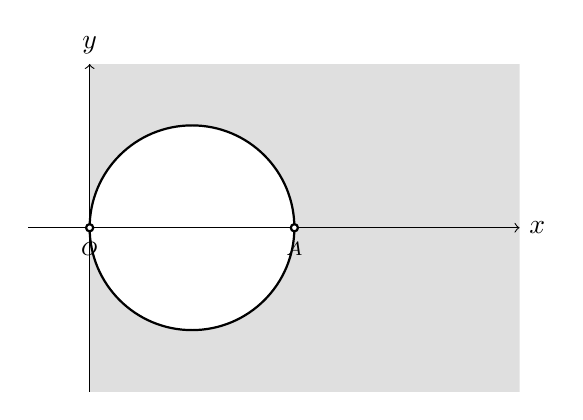
\begin{tikzpicture}[scale=1.3]
  \def\a{2}
  \begin{scope}
    \clip (0,-1.6) rectangle (4.2,1.6);
    \fill[gray!25] (0,-1.6) rectangle (4.2,1.6);
    \fill[white] (\a/2,0) circle (\a/2);
  \end{scope}
  \draw[->] (-0.6,0) -- (4.2,0) node[right]{$x$};
  \draw[->] (0,-1.6) -- (0,1.6) node[above]{$y$};
  \draw[thick] (\a/2,0) circle (\a/2);
  \filldraw[white,draw=black,thick] (0,0) circle (0.035);
  \filldraw[white,draw=black,thick] (\a,0) circle (0.035);
  \node[below] at (0,-0.05) {\scriptsize$O$};
  \node[below] at (\a,-0.05) {\scriptsize$A$};
\end{tikzpicture}
\caption{領域$D$（斜線部，境界を含み$O,A$の2点のみ除く；$x<0$の部分は含まない）}
\end{figure}
\end{proof}

\end{document}
